\section{优化问题的表述}
\label{sec:opt-prob-formulation}

要找“最低点”，先得说清在哪些位置里找、按什么高度比较。本节先规定一个优化问题由哪些对象组成，再定义最优值与最优解，并区分只和附近比较的局部最优与和所有候选比较的全局最优。最后引入扩展实值写法，把“哪些位置允许站”并入目标函数本身；这种写法只统一表示方式，不改变问题的解。

\subsection{变量、目标与可行域}
\label{sec:opt-prob-variables}

\paragraph{资源分配}
一个车间生产两种产品，产量分别记为$x_1,x_2$（单位：批）。每批产品一的利润为$3$，产品二为$2$。生产受两种资源限制：每批产品各用$1$个工时，每天共有$4$个工时；每批产品一用$2$份原料、产品二用$1$份，每天共有$6$份原料。产量不能为负。可以调整的量是$\bm x=(x_1,x_2)^\top\in\mathbb R^2$，要比较的是利润$3x_1+2x_2$，允许的产量组合满足
\begin{equation}
  x_1+x_2\leq4,\qquad 2x_1+x_2\leq6,\qquad x_1\geq0,\qquad x_2\geq0.
  \label{eq:opt-prob-resource}
\end{equation}
一般地，$d$种产品、$m$种资源时，变量是$\bm x\in\mathbb R^d$，利润系数$\bm c\in\mathbb R^d$，第$i$种资源每单位产品$j$的用量为$G_{i,j}$，资源上限为$h_i$；约束写成$\bm G\bm x\leq\bm h$与$\bm x\geq\bm 0$，其中$\bm G\in\mathbb R^{m\times d}$，向量不等式逐个坐标理解。

利润要最大化，而本书统一讨论最小化。二者只差一个符号：最大化$3x_1+2x_2$与最小化$f(\bm x)=-(3x_1+2x_2)$选出相同的产量，最大利润等于最小值的相反数。一般地，$\max_{\bm x\in C}p(\bm x)=-\min_{\bm x\in C}\bigl(-p(\bm x)\bigr)$，取得两侧的点也相同。这个转换是记号上的约定，不涉及任何求解技巧。

图~\ref{fig:opt-prob-resource-region}把约束~\eqref{eq:opt-prob-resource}画在平面上：四条直线围出一个四边形，它就是“允许站的地”。虚线是利润相等的产量组合，沿箭头方向平移时利润增大。读者可以从图中看到，利润为$10$的直线恰好擦过四边形的一个角$(2,2)$，再往外移就离开了允许区域。这一观察还不是证明；第~\ref{sec:opt-prob-optimal-value}小节将给出一个两行的论证，第~\ref{chap:opt-linear-programming}章再把“在角点处寻找”发展成一般方法。

\begin{figure}[!htbp]
  \centering
  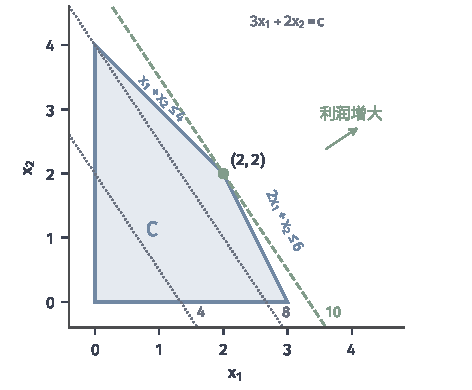
\includegraphics[width=80mm]{figures/03-optimization-evolution-and-signals/01-optimization/matplotlib/c1-resource-region/figure.pdf}
  \caption{资源分配问题的可行域与利润等值线。蓝色四边形$C$由$x_1+x_2\leq4$、$2x_1+x_2\leq6$与$\bm x\geq\bm 0$围成，顶点为$(0,0),(3,0),(2,2),(0,4)$。灰色点线与绿色虚线是$3x_1+2x_2=c$在$c=4,8,10$时的直线（数值标在横轴下方）；利润为$10$的直线只与$C$交于顶点$(2,2)$。}
  \label{fig:opt-prob-resource-region}
\end{figure}

\paragraph{带正则项的最小二乘}
第二个任务来自数据拟合。设有$n$个观测、$d$个待定参数，设计矩阵$\bm A\in\mathbb R^{n\times d}$的第$i$行记录第$i$个观测的输入，$\bm b\in\mathbb R^n$记录观测值。参数$\bm x\in\mathbb R^d$给出的预测为$\bm A\bm x$，我们最小化
\begin{equation}
  f(\bm x)=\frac12\lVert\bm A\bm x-\bm b\rVert_2^2+\frac{\lambda}{2}\lVert\bm x\rVert_2^2,
  \qquad\lambda\geq0.
  \label{eq:opt-prob-ridge}
\end{equation}
第一项是预测与观测之差的平方和的一半，第二项是正则项，$\lambda$是正则系数。若业务要求参数非负，还可以加上硬约束$\bm x\geq\bm 0$。三者改变的东西不同：换掉数据误差会改变“拟合得好”的含义；正则项给大参数计价，改变的是候选之间的比较；硬约束则直接改变哪些候选允许参加比较。正则项再大也只是让违规代价变高，硬约束却把违规候选排除在外，这一区别在第~\ref{sec:opt-prob-extended-value}小节会再次出现。

本章反复使用一个最小的实例：只有一个观测$n=1$，两个参数$d=2$，$\bm A=(1\ \ 1)$，$\bm b=2$。它的含义是“只测到了两个量之和等于$2$”，于是
\[
  f(\bm x)=\frac12(x_1+x_2-2)^2+\frac{\lambda}{2}(x_1^2+x_2^2).
\]
这个实例虽小，却足以展示解不唯一、正则化恢复唯一性以及误差度量之间的差异。

\paragraph{问题的统一写法}
两个任务都可以写成同一个形式：在集合$C\subseteq\mathbb R^d$中选$\bm x$，使$f(\bm x)$尽量小，
\begin{equation}
  \min_{\bm x\in C}f(\bm x).
  \label{eq:opt-prob-general}
\end{equation}

\begin{definition}[优化问题]
\label{def:opt-prob-problem}
给定集合$C\subseteq\mathbb R^d$与函数$f:C\to\mathbb R$，问题~\eqref{eq:opt-prob-general}称为一个\term{优化问题}（optimization problem）。$\bm x$称为\term{决策变量}（decision variable），$f$称为\term{目标函数}（objective function），$C$称为\term{可行域}（feasible set），$C$中的点称为\term{可行点}（feasible point）。可行域常由不等式$g_i(\bm x)\leq0$（$i=1,\dots,m$）和等式$h_j(\bm x)=0$（$j=1,\dots,p$）描述，这些条件称为约束。
\end{definition}

资源分配中，$C$是约束~\eqref{eq:opt-prob-resource}围出的四边形，$f(\bm x)=-(3x_1+2x_2)$，约束可写成$g_1(\bm x)=x_1+x_2-4$、$g_2(\bm x)=2x_1+x_2-6$、$g_3(\bm x)=-x_1$、$g_4(\bm x)=-x_2$均不大于零。最小二乘中，$C=\mathbb R^d$或加上非负约束后的$\{\bm x:\bm x\geq\bm 0\}$，$f$是式~\eqref{eq:opt-prob-ridge}。

$C$与$f$必须一起给定，问题才算确定。同样是最小二乘，把$\lambda$从$0$改成$0.5$，或把$C$从全空间改成非负象限，得到的是不同的问题，答案也可能不同。本小节只把模型固定下来；下一小节规定怎样称呼它的解。

\subsection{最优值与最优解}
\label{sec:opt-prob-optimal-value}

“最低点”包含两个不同的问题：最低的高度是多少，以及在哪里取得。前者是一个数，后者是一个位置。从比较所有可行点的目标值出发，可以分别定义它们。

\begin{definition}[最优值与最优解]
\label{def:opt-prob-optimal-value}
问题~\eqref{eq:opt-prob-general}的\term{最优值}（optimal value）是
\[
  f^\star=\inf_{\bm x\in C}f(\bm x)\in[-\infty,+\infty],
\]
并约定空集上的下确界为$+\infty$。若$C=\varnothing$，称问题\term{不可行}（infeasible）；若$C\neq\varnothing$且$f^\star=-\infty$，称问题\term{无下界}（unbounded below）。可行点$\bm x^\star$若满足$f(\bm x^\star)=f^\star$，称为\term{最优解}（optimal solution）或最小点，全体最优解组成的集合记为$\argmin_{\bm x\in C}f$。若这个集合非空，就说最优值被达到。
\end{definition}

于是要回答三个判断：问题是否可行，是否下有界，最优值是否被达到。前两项决定$f^\star$是不是一个有限实数，第三项决定是否真有一个可行点能报告出来。写下$\min_{\bm x\in C}f(\bm x)$只表示提出了求最小值的任务；声称“最小值等于某个数”，才同时断言了这个值被某个可行点取得。

\paragraph{资源分配的最优解}
回到资源分配。对任意可行点，把两条资源约束相加：
\[
  3x_1+2x_2=(x_1+x_2)+(2x_1+x_2)\leq4+6=10.
\]
所以利润不超过$10$，即$f(\bm x)\geq-10$。等号成立当且仅当两条资源约束同时取等号，即$x_1+x_2=4$且$2x_1+x_2=6$，解得$\bm x=(2,2)$，它满足非负约束，因而可行。于是$f^\star=-10$，最优解集合恰好是$\{(2,2)\}$。这个论证同时给出了最优值的下界和一个达到下界的可行点，二者合起来才证明了“$(2,2)$最优”；第~\ref{chap:opt-linear-programming}章会说明，这样的“约束加权组合”正是线性规划最优性证书的雏形。

\paragraph{三种失败}
并非每个问题都这样顺利。图~\ref{fig:opt-prob-failure-modes}画出三种情形，失败分别发生在不同对象上。同时要求$x\leq0$与$x\geq1$时，$C=\varnothing$，问题不可行，失败在可行域。在$C=\mathbb R$上最小化$f(x)=x$时，取$x=-k$得$f=-k\to-\infty$，问题无下界，失败在目标没有底。在$C=\mathbb R$上最小化$f(x)=e^x$时，$e^x>0$且$e^{-k}\to0$，所以$f^\star=0$是有限实数，但没有$x$使$e^x=0$，最优解集合为空；这时可行性与下有界都成立，失败在“达到”这一步。第三种情形最容易被忽略：只报告$f^\star=0$而不说明未达到，读者会误以为存在一个最优参数。

\begin{figure*}[!htbp]
  \centering
  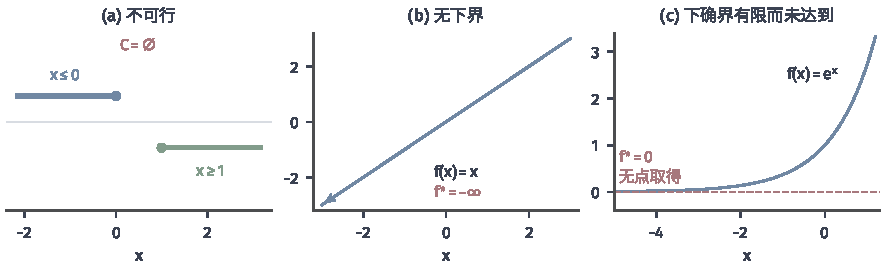
\includegraphics[width=150mm]{figures/03-optimization-evolution-and-signals/01-optimization/matplotlib/c1-failure-modes/figure.pdf}
  \caption{优化问题没有最优解的三种方式。(a) 约束$x\leq0$（蓝）与$x\geq1$（绿）没有公共点，可行域为空。(b) $f(x)=x$在实轴上沿箭头方向无限下降，最优值为$-\infty$。(c) $f(x)=e^x$的值趋于红色虚线$0$却永不等于$0$：最优值有限，但没有可行点取得它。}
  \label{fig:opt-prob-failure-modes}
\end{figure*}

到目前为止，我们假定目标在每个可行点上取有限实数值。第~\ref{sec:opt-prob-extended-value}小节将允许目标取$+\infty$，届时再检查这些定义是否仍然适用。

\subsection{局部最优与全局最优}
\label{sec:opt-prob-local-global}

站在地形中的一个洼地底部，向四周看处处都更高，但山那边可能还有更深的谷。只和附近比较，与和所有可行点比较，是两个不同的要求。下面用欧氏开球$B(\bm x,r)=\{\bm y:\lVert\bm y-\bm x\rVert_2<r\}$刻画“附近”。

\begin{definition}[局部最优与全局最优]
\label{def:opt-prob-local-global}
设$\bm x^\star\in C$。若$f(\bm x^\star)\leq f(\bm x)$对所有$\bm x\in C$成立，称$\bm x^\star$为\term{全局最优解}（global minimizer）。若存在$r>0$，使$f(\bm x^\star)\leq f(\bm x)$对所有$\bm x\in C\cap B(\bm x^\star,r)$成立，称$\bm x^\star$为\term{局部最优解}（local minimizer）；若进一步对所有$\bm x\in C\cap B(\bm x^\star,r)$、$\bm x\neq\bm x^\star$有严格不等式，称为\term{严格局部最优解}（strict local minimizer）。
\end{definition}

全局最优解就是定义~\ref{def:opt-prob-optimal-value}中的最优解。局部比较的范围是$C\cap B(\bm x^\star,r)$而不是整个球：可行域边界上的点只需与球内的可行点比较，球中伸出可行域的部分不参加比较。

\begin{example}[边界上的最优与多个洼地]
\label{ex:opt-prob-local-global}
取$f(x)=x^4/4-x^3/3-x^2$，可行域$C=[-1.5,1.5]$。导数$f'(x)=x^3-x^2-2x=x(x-2)(x+1)$在$x=-1,0,2$处为零。计算得$f(-1)=-5/12\approx-0.417$，$f(0)=0$，$f(1.5)\approx-2.109$，$f(-1.5)\approx0.141$。由$f'$的符号，$f$在$[-1.5,-1]$上递减、在$[-1,0]$上递增、在$[0,1.5]$上递减。所以$x=-1$附近的可行点函数值都不低于$-5/12$，它是局部最优解；而$C$上的最小值只能出现在$x=-1$或右端点$x=1.5$，后者更低，因此$x=1.5$是$C$上的全局最优解。在这个边界点处$f'(1.5)=-1.875\neq0$：函数仍在向右下降，只是可行域不允许再往右走。若去掉约束，最低点会移到$C$之外的$x=2$，$f(2)=-8/3$。
\end{example}

图~\ref{fig:opt-prob-local-global}画出这个例子。浅蓝色带是可行域，读者应注意三件事：$x=-1$是一个洼地底部，却不是最低处；全局最优落在可行域的边界上，那里的切线并不水平；可行域之外还有更低的点，它与问题无关。这说明局部最优与全局最优必须按定义区分，也说明不能先用“导数为零”代替最优解的定义——第~\ref{sec:opt-prob-optimality}节会看到，导数为零只在可行域内部的点上才是必要条件。

\begin{figure}[!htbp]
  \centering
  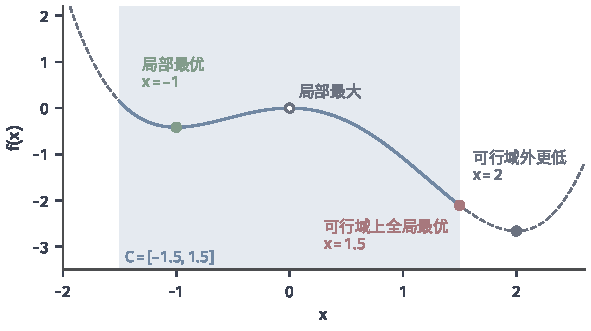
\includegraphics[width=100mm]{figures/03-optimization-evolution-and-signals/01-optimization/matplotlib/c1-local-global/figure.pdf}
  \caption{$f(x)=x^4/4-x^3/3-x^2$在可行域$C=[-1.5,1.5]$（浅蓝色带）上的局部与全局最优。蓝色实线是$C$上的图像，虚线是$C$外的部分。绿点$x=-1$是局部最优解，红点$x=1.5$是$C$上的全局最优解（该处导数为$-1.875$），空心点$x=0$是局部最大点，灰点$x=2$是$C$之外的更低点。}
  \label{fig:opt-prob-local-global}
\end{figure}

\paragraph{严格、唯一与多个等值解}
严格局部最优解在一个小邻域内是唯一的最低点，但这不排除远处还有同样低或更低的点。$f(x)=(x^2-1)^2$在$x=\pm1$处都取到全局最小值$0$，两点各自都是严格局部最优解，全局最优解却有两个。全局最优解唯一，是比“每个最优解都是严格局部最优”更强的整体性质。

\paragraph{参数不唯一而预测相同}
最小二乘实例在$\lambda=0$时给出一个更有实际意义的情形。此时$f(\bm x)=\tfrac12(x_1+x_2-2)^2\geq0$，凡满足$x_1+x_2=2$的点都使$f=0$，因而都是全局最优解；最优解集合是一整条直线（图~\ref{fig:opt-prob-ls-sublevel}(a)中的绿色虚线）。直线上任意两个参数，例如$(1,1)$与$(3,-1)$，对唯一的观测给出相同的预测$\bm A\bm x=2$。数据只约束了$x_1+x_2$，没有约束$x_1-x_2$；在给定样本上，选哪个参数都一样好，但若用它们去预测新的输入$(1,0)$，结果分别是$1$和$3$。参数不唯一不是计算的失败，而是问题本身没有提供区分它们的信息。

\subsection{扩展实值目标}
\label{sec:opt-prob-extended-value}

到目前为止，可行域和目标是两个分开的对象。后续章节常常要把几种代价相加，或者把约束子问题交给同一个工具处理，那时“$f$加上一个集合”很不方便。一个自然的想法是：让不可行的点取一个大到不可能被选中的值，从而不参加比较。取任何有限的大数都不够保险，于是允许取$+\infty$。

\begin{definition}[扩展实值函数、有效定义域与指示函数]
\label{def:opt-prob-extended}
取值于$\mathbb R\cup\{+\infty\}$的函数$f:\mathbb R^d\to\mathbb R\cup\{+\infty\}$称为\term{扩展实值函数}（extended real-valued function）。它的\term{有效定义域}（effective domain）是$\operatorname{dom}f=\{\bm x:f(\bm x)<+\infty\}$。若$\operatorname{dom}f\neq\varnothing$，称$f$为\term{适当函数}（proper function）。集合$C\subseteq\mathbb R^d$的\term{指示函数}（indicator function）为
\[
  \iota_C(\bm x)=\begin{cases}0,&\bm x\in C,\\+\infty,&\bm x\notin C.\end{cases}
\]
扩展实值目标的最优值仍为$f^\star=\inf_{\bm x\in\mathbb R^d}f(\bm x)$，最优解集合规定为$\argmin f=\{\bm x\in\operatorname{dom}f:f(\bm x)=f^\star\}$。
\end{definition}

这里不允许取$-\infty$，所以“适当”只需要求至少有一点取有限值。最优解集合只在有效定义域中寻找，这是为了排除一种错觉：若$f$处处为$+\infty$，则$f^\star=+\infty$，每一点都“等于最优值”，但没有一个点是可用的答案。

\paragraph{统一写法保留了什么}
给定非空$C$和$C$上的实值目标$f_0$，令$F(\bm x)=f_0(\bm x)$（$\bm x\in C$），$F(\bm x)=+\infty$（$\bm x\notin C$），也记作$F=f_0+\iota_C$。逐项核对：$\operatorname{dom}F=C$，所以$F$适当，有限值候选恰好是可行点；$F$与$f_0$在可行点上取值相同，在其余点取$+\infty$，不影响下确界，所以$\inf F=\inf_Cf_0$；最优解只在$\operatorname{dom}F=C$中找，因而$\argmin F=\argmin_Cf_0$。约束问题与它的扩展实值写法有相同的最优值和相同的最优解，“达到”与否也一致。若$C=\varnothing$，则$F\equiv+\infty$，不适当，应报告不可行，而不能说每一点都最优。

\paragraph{指示函数不同于惩罚}
要区分三种看起来相近的对象。指示函数$\iota_C$取$0$与$+\infty$，它把违规点彻底排除。取$0$与$1$的集合示性函数$\mathbb 1_C$（在$C$上为$1$、在$C$外为$0$）只是一个普通的有界函数，把它加到目标上不会禁止任何点。有限惩罚则给违规程度定价，例如在$C=\{x:x\leq1\}$上最小化$(x-2)^2$时，改用
\[
  (x-2)^2+\max\{0,x-1\}
\]
代替约束。当$x>1$时，该函数的导数$2(x-2)+1$在$x=1.5$处为零，此处函数值$0.25+0.5=0.75$小于可行最优值$(1-2)^2=1$，所以惩罚问题的最小点$x=1.5$违反了约束。图~\ref{fig:opt-prob-extended-value}画出了这一差别：惩罚只是“不喜欢”违规，指示函数才真正禁止违规。惩罚系数多大才能恢复约束、怎样逐步加大惩罚，是第~\ref{chap:constrained-optimization}章的话题。

\begin{figure}[!htbp]
  \centering
  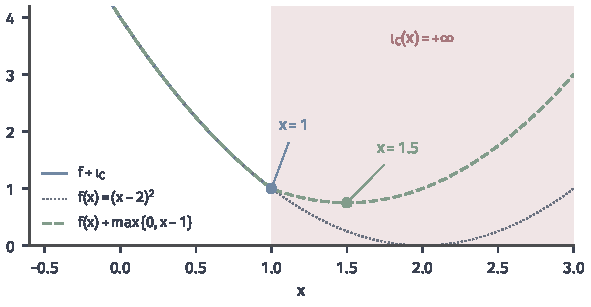
\includegraphics[width=100mm]{figures/03-optimization-evolution-and-signals/01-optimization/matplotlib/c1-extended-value/figure.pdf}
  \caption{指示函数与有限惩罚。目标$f(x)=(x-2)^2$（灰色点线），约束$x\leq1$。蓝线是$f+\iota_C$：在粉色区域$x>1$中取值$+\infty$，最小点为$x=1$、最小值为$1$。绿色虚线是加上惩罚$\max\{0,x-1\}$后的目标，最小点为$x=1.5$、最小值为$0.75$，落在约束之外。}
  \label{fig:opt-prob-extended-value}
\end{figure}

此后需要时，我们把约束问题~\eqref{eq:opt-prob-general}直接写成扩展实值目标的无约束最小化；两种写法描述同一个问题。
